\documentclass[a4paper]{article}
\usepackage{listings}
\usepackage{geometry}
\usepackage[parfill]{parskip}
\usepackage[bottom]{footmisc}

\usepackage[bookmarks=true, bookmarksopen=true]{hyperref}
\usepackage{bookmark}
\usepackage{enumitem}
\usepackage{color}
\definecolor{linkcolour}{rgb}{0,0.2,0.6}
\hypersetup{colorlinks, breaklinks, urlcolor=linkcolour, linkcolor=linkcolour}

\usepackage{amsmath, bm}
\newcommand{\norm}[1]{\left\lVert#1\right\rVert}

\usepackage{csvsimple}

% Font
\usepackage{fontspec}
\setmainfont{GFS Artemisia}

\renewcommand{\figureautorefname}{Σχήμα}
\renewcommand{\tableautorefname}{Πίνακας}

% Images
\usepackage{graphicx}
\graphicspath{{../../figures/kpca/}}
\usepackage[font={footnotesize,it}]{caption}
\usepackage[font={footnotesize}]{subcaption}
\renewcommand{\thesubfigure}{\Roman{subfigure}}
\usepackage{float}

% English-Greek use
\usepackage{polyglossia}
\setmainlanguage{greek}
\setotherlanguage{english}

% References
\usepackage[backend=biber,style=alphabetic]{biblatex}
\addbibresource{references.bib}

\geometry{
 a4paper,
 total={170mm,257mm},
 left=20mm,
 top=20mm,
}

\title{Υπολογιστική Νοημοσύνη - Στατιστική μάθηση \\ Δεύτερη Εργασία}
\author{Κωστινούδης Ευάγγελος \\ΑΕΜ: 112}
\date{\today}

\begin{document}
\maketitle
\pagenumbering{gobble}
\newpage
\pagenumbering{arabic}

\section{Περιγραφή προβλήματος που επιλέχτηκε}

Οι βάσεις που επιλέχτηκαν, οι οποίες είναι ίδιες με την προηγούμενη εργασία,
είναι:

\begin{enumerate}
\item \href{http://yann.lecun.com/exdb/mnist/}{MNIST}
\item \href{https://www.cs.toronto.edu/~kriz/cifar.html}{Cifar-10}
\end{enumerate}


\section{Υλοποίηση}

Ο αλγόριθμος KPCA plus LDA υλοποιήθηκε σύμφωνα με το \cite{kpca_lda} και η
υλοποίηση βρίσκεται στο αρχείο \textit{kpca\_plus\_lda.py}.

Για την εκπαίδευση των μοντέλων χρησιμοποιούνται τα δεδομένα εκπαίδευσης που
δίνονται από τις δύο βάσεις που αναφέρονται παραπάνω. Αντίστοιχα
χρησιμοποιούνται τα δεδομένα ελέγχουν για τον έλεγχο των μοντέλων.

\subsection{Επιλογή δειγμάτων}

Επειδή ο αλγόριθμος KPCA plus LDA έχει πολυπλοκότητα χώρου $O(n_{sample})$,
γεγονός που καθιστά αδύνατο να τρέξει στο σύστημα μου, επιλέχτηκε ένα υποσύνολο
των δεδομένων εκπαίδευσης. Συγκεκριμένα, και για τις δύο βάσεις,
χρησιμοποιήθηκαν 1.200 δήγματα για κάθε κλάση δηλαδή 12.000 συνολικά για το
σύνολο εκπαίδευσης. Αυτό φαίνεται και από το \autoref{fig:hist}, όπου
παρουσιάζονται τα ιστογράμματα των κλάσεων για τα δεδομένα εκπαίδευσης πριν και
μετά την υποδειγματοληψία.

\begin{figure}[H]
    \centering

    \begin{subfigure}[t]{0.48\linewidth}
    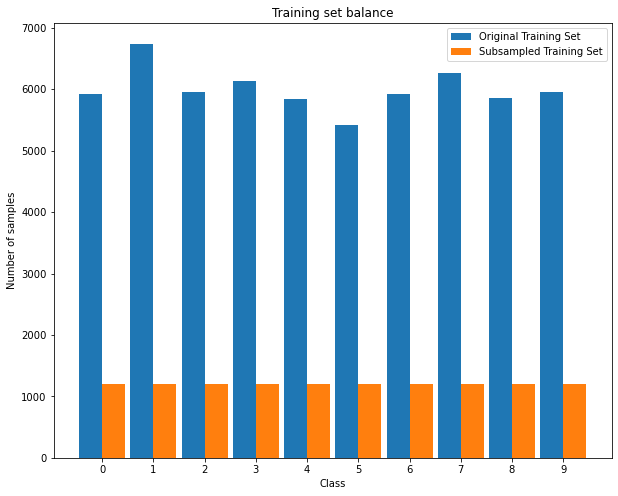
\includegraphics[width=\linewidth]{mnist/training_freq.png}
    \caption{Ιστόγραμμα κλάσεων πριν και μετά την υποδειγματοληψία για τη βάση
    MNIST}
    \label{fig:hist1}
    \end{subfigure}
    \begin{subfigure}[t]{0.48\linewidth}
    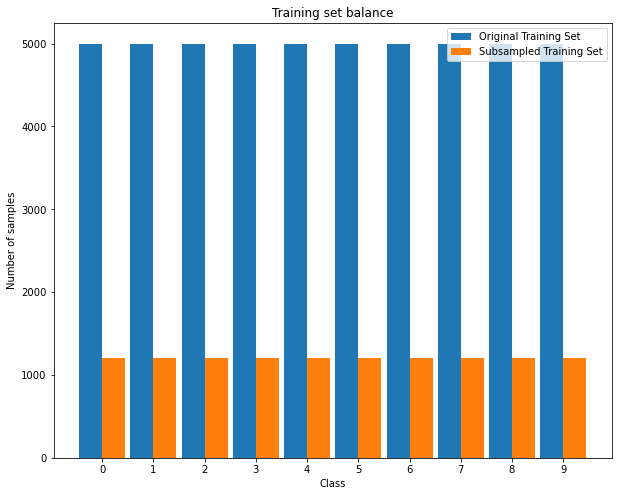
\includegraphics[width=\linewidth]{cifar/training_freq.png}
    \caption{Ιστόγραμμα κλάσεων πριν και μετά την υποδειγματοληψία για τη βάση
        Cifar-10}
    \end{subfigure}

    \caption{Ιστογράμματα κλάσεων για τις βάσεις δεδομένων}
    \label{fig:hist}
\end{figure}

\subsection{Προεπεξεργασία δεδομένων}

Η μόνη προεπεξεργασία που έγινε στα δεδομένα πριν την χρήση τους στον αλγόριθμο
KPCA plus LDA είναι ο μετασχηματισμός των δεδομένων στο διάστημα $[0,1]$ για
κάθε χαρακτηριστικό των δεδομένων.

\subsection{Επιλογή παραμέτρων}

Για την εύρεση των καλύτερων παραμέτρων το σύνολο εκπαίδευσης χωρίστηκε σε
σύνολο εκπαίδευσης και επικύρωσης, όπου το σύνολο εκπαίδευσης αποτελείται από
7.000 δείγματα και το σύνολο επικύρωσης από 5.000 δείγματα και για τις δύο
βάσεις.

Όσο αφορά τον αλγόριθμο KPCA plus LDA οι παράμετροι αφορούν τον πυρήνα και τις
επιμέρους παραμέτρους. Για τη βάση MNIST οι παράμετροι είναι:

\begin{enumerate}
    \item Γραμμικός πυρήνας.
    \item Πολυωνυμικός πυρήνας: $d: 2, \gamma: (0.1, 1, 10)$.
    \item RBF πυρήνας: $\gamma: (0.05, 0.1, 0.5)$.
    \item Σιγμοειδής πυρήνας: $\gamma: (0.00001, 0.0001, 0.001$).
\end{enumerate}

Και για τη βάση Cifar-10:

\begin{enumerate}
    \item Γραμμικός πυρήνας.
    \item Πολυωνυμικός πυρήνας: $d: 2, \gamma: (0.01, 0.1, 1)$.
    \item RBF πυρήνας: $\gamma: (0.001, 0.01, 0.1)$.
    \item Σιγμοειδής πυρήνας: $\gamma: (0.00001, 0.0001, 0.001$).
\end{enumerate}

Οι παράμετροι για κάθε πυρήνα είναι:

\begin{enumerate}
    \item Πολυωνυμικός πυρήνας: $K(\bm{x}_i,\bm{x}_j) = (\gamma \bm{x}_i^T
        \bm{x}_j)^d$.
    \item RBF πυρήνας: $K(\bm{x}_i,\bm{x}_j) = exp(-\gamma \norm{\bm{x}_i -
        \bm{x}_j}^2)$.
    \item Σιγμοειδή πυρήνας: $K(\bm{x}_i,\bm{x}_j) = tanh(\gamma \bm{x}_i^T
        \bm{x}_j)$.
\end{enumerate}

Για την ταξινόμηση χρησιμοποιήθηκαν οι μέθοδοι πλησιέστερων γειτόνων (Nearest
Neighbors) και πλησιέστερου κέντρου κλάσης (Nearest Class Centroid). Για το
μοντέλο πλησιέστερων γειτόνων και για τις δύο βάσεις χρησιμοποιήθηκε
$n\_neighbors: (1, 3, 5, 10, 15)$ όπου $n\_neighbors$ ο αριθμός των γειτόνων.

Για το μοντέλο πλησιέστερων γειτόνων, για την απόσταση των γειτόνων
χρησιμοποιήθηκε η fused απόσταση που δίνεται στο \cite{kpca_lda} με $\theta =1$.
Για το μοντέλο του πλησιέστερου κέντρου κλάσης χρησιμοποιήθηκαν τα regular and
irregular discriminant features που παρουσιάζονται στο \cite{kpca_lda}. Το
μέγεθος του διανύσματος των χαρακτηριστικών είναι 18 από τα οποία 9 αφορούν τα
regular και 9 irregular discriminant features και για τις δύο βάσης.


\section{Αποτελέσματα}

Τα πειράματα εκτελέστηκαν σε επεξεργαστή Intel i7-4510U και 8GB μνήμη. Επίσης,
για τις μετρικές precision, recall και F1 χρησιμοποιήθηκε η macro εκδοχή τους
που είναι ο μέσος όρος των μετρικών αυτών για κάθε κλάση.

\subsection{Επιλογή παραμέτρων}

\subsubsection{MNIST}

\paragraph{Πλησιέστερων γειτόνων}

Στο \autoref{tab:mnist_knn_val} παρουσιάζονται τα αποτελέσματα στο σύνολο
επικύρωσης. Παρατηρείται ότι το καλύτερο μοντέλο βάση της μετρικής accuracy
είναι αυτό με RBF πυρήνα, $\gamma = 0.05$ και αριθμό γειτόνων 1.

\begin{table}[H]
\centering
\begin{tabular}{|l|c|c|c|c|c|}
\hline
\textbf{Model}                                                                & \textbf{Best n} & \textbf{Accuracy} & \textbf{Precision} & \textbf{Recall} & \textbf{F1} \\ \hline
kernel: linear                                                                & 1               & 0,1               & 0,01               & 0,1             & 0,0182      \\ \hline
\begin{tabular}[c]{@{}l@{}}kernel: poly\\ degree: 2\\ gamma: 0.1\end{tabular} & 1               & 0,2468            & 0,2038             & 0,2468          & 0,1831      \\ \hline
\begin{tabular}[c]{@{}l@{}}kernel: poly\\ degree: 2\\ gamma: 1\end{tabular}   & 3               & 0,2944            & 0,3749             & 0,2944          & 0,23        \\ \hline
\begin{tabular}[c]{@{}l@{}}kernel: poly\\ degree: 2\\ gamma: 10\end{tabular}  & 1               & 0,1               & 0,01               & 0,1             & 0,0182      \\ \hline
\begin{tabular}[c]{@{}l@{}}kernel: rbf\\ gamma: 0.05\end{tabular}             & 1               & 0,965             & 0,9652             & 0,965           & 0,965       \\ \hline
\begin{tabular}[c]{@{}l@{}}kernel: rbf\\ gamma: 0.1\end{tabular}              & 1               & 0,8762            & 0,9264             & 0,8762          & 0,8892      \\ \hline
\begin{tabular}[c]{@{}l@{}}kernel: rbf\\ gamma: 0.5\end{tabular}              & 10              & 0,2628            & 0,9015             & 0,2628          & 0,2604      \\ \hline
\begin{tabular}[c]{@{}l@{}}kernel: sigmoid\\ gamma: 1e-05\end{tabular}        & 3               & 0,1002            & 0,06               & 0,1002          & 0,0186      \\ \hline
\begin{tabular}[c]{@{}l@{}}kernel: sigmoid\\ gamma: 0.0001\end{tabular}       & 1               & 0,1               & 0,01               & 0,1             & 0,0182      \\ \hline
\begin{tabular}[c]{@{}l@{}}kernel: sigmoid\\ gamma: 0.001\end{tabular}        & 3               & 0,1574            & 0,0812             & 0,1574          & 0,0829      \\ \hline
\end{tabular}
\caption{Αποτελέσματα επιλογής παραμέτρων για την μέθοδο πλησιέστερων γειτόνων
    και τη βάση MNIST}
\label{tab:mnist_knn_val}
\end{table}


\paragraph{Πλησιέστερου κέντρου κλάσης}

Στο \autoref{tab:mnist_nc_val} παρουσιάζονται τα αποτελέσματα στο σύνολο
επικύρωσης. Παρατηρείται ότι το καλύτερο μοντέλο βάση της μετρικής accuracy
είναι αυτό με RBF πυρήνα και $\gamma = 0.05$.

\begin{table}[H]
\centering
\begin{tabular}{|l|c|c|c|c|}
\hline
\textbf{Model}                                                                & \textbf{Accuracy} & \textbf{Precision} & \textbf{Recall} & \textbf{F1} \\ \hline
kernel: linear                                                                & 0,195             & 0,1683             & 0,195           & 0,098       \\ \hline
\begin{tabular}[c]{@{}l@{}}kernel: poly\\ degree: 2\\ gamma: 0.1\end{tabular} & 0,9156            & 0,9254             & 0,9156          & 0,9161      \\ \hline
\begin{tabular}[c]{@{}l@{}}kernel: poly\\ degree: 2\\ gamma: 1\end{tabular}   & 0,7542            & 0,8715             & 0,7542          & 0,7506      \\ \hline
\begin{tabular}[c]{@{}l@{}}kernel: poly\\ degree: 2\\ gamma: 10\end{tabular}  & 0,1               & 0,01               & 0,1             & 0,0182      \\ \hline
\begin{tabular}[c]{@{}l@{}}kernel: rbf\\ gamma: 0.05\end{tabular}             & 0,9292            & 0,932              & 0,9292          & 0,9299      \\ \hline
\begin{tabular}[c]{@{}l@{}}kernel: rbf\\ gamma: 0.1\end{tabular}              & 0,6912            & 0,8712             & 0,6912          & 0,7356      \\ \hline
\begin{tabular}[c]{@{}l@{}}kernel: rbf\\ gamma: 0.5\end{tabular}              & 0,1526            & 0,1723             & 0,1526          & 0,0916      \\ \hline
\begin{tabular}[c]{@{}l@{}}kernel: sigmoid\\ gamma: 1e-05\end{tabular}        & 0,1152            & 0,206              & 0,1152          & 0,0453      \\ \hline
\begin{tabular}[c]{@{}l@{}}kernel: sigmoid\\ gamma: 0.0001\end{tabular}       & 0,1278            & 0,1024             & 0,1278          & 0,0614      \\ \hline
\begin{tabular}[c]{@{}l@{}}kernel: sigmoid\\ gamma: 0.001\end{tabular}        & 0,133             & 0,2562             & 0,133           & 0,0739      \\ \hline
\end{tabular}
\caption{Αποτελέσματα επιλογής παραμέτρων για την μέθοδο πλησιέστερου κέντρου
    κλάσης και τη βάση MNIST}
\label{tab:mnist_nc_val}
\end{table}

\subsubsection{Cifar-10}

\paragraph{Πλησιέστερων γειτόνων}

Στο \autoref{tab:cifar_knn_val} παρουσιάζονται τα αποτελέσματα στο σύνολο
επικύρωσης. Παρατηρείται ότι το καλύτερο μοντέλο βάση της μετρικής accuracy
είναι αυτό με RBF πυρήνα, $\gamma = 0.01$ και αριθμό γειτόνων 15.

\begin{table}[H]
\centering
\begin{tabular}{|l|c|c|c|c|c|}
\hline
\textbf{Model}                                                                 & \textbf{Best n} & \textbf{Accuracy} & \textbf{Precision} & \textbf{Recall} & \textbf{F1} \\ \hline
kernel: linear                                                                 & 1               & 0,1               & 0,01               & 0,1             & 0,0182      \\ \hline
\begin{tabular}[c]{@{}l@{}}kernel: poly\\ degree: 2\\ gamma: 0.01\end{tabular} & 1               & 0,1               & 0,01               & 0,1             & 0,0182      \\ \hline
\begin{tabular}[c]{@{}l@{}}kernel: poly\\ degree: 2\\ gamma: 0.1\end{tabular}  & 3               & 0,1058            & 0,0278             & 0,1058          & 0,029       \\ \hline
\begin{tabular}[c]{@{}l@{}}kernel: poly\\ degree: 2\\ gamma: 1\end{tabular}    & 1               & 0,1               & 0,01               & 0,1             & 0,0182      \\ \hline
\begin{tabular}[c]{@{}l@{}}kernel: rbf\\ gamma: 0.001\end{tabular}             & 1               & 0,1               & 0,01               & 0,1             & 0,0182      \\ \hline
\begin{tabular}[c]{@{}l@{}}kernel: rbf\\ gamma: 0.01\end{tabular}              & 15              & 0,4198            & 0,5173             & 0,4198          & 0,4233      \\ \hline
\begin{tabular}[c]{@{}l@{}}kernel: rbf\\ gamma: 0.1\end{tabular}               & 10              & 0,1868            & 0,3889             & 0,1868          & 0,1686      \\ \hline
\begin{tabular}[c]{@{}l@{}}kernel: sigmoid\\ gamma: 1e-05\end{tabular}         & 1               & 0,1               & 0,01               & 0,1             & 0,0182      \\ \hline
\begin{tabular}[c]{@{}l@{}}kernel: sigmoid\\ gamma: 0.0001\end{tabular}        & 1               & 0,1               & 0,01               & 0,1             & 0,0182      \\ \hline
\begin{tabular}[c]{@{}l@{}}kernel: sigmoid\\ gamma: 0.001\end{tabular}         & 1               & 0,1               & 0,01               & 0,1             & 0,0182      \\ \hline
\end{tabular}
\caption{Αποτελέσματα επιλογής παραμέτρων για την μέθοδο πλησιέστερων γειτόνων
    και τη βάση Cifar-10}
\label{tab:cifar_knn_val}
\end{table}


\paragraph{Πλησιέστερου κέντρου κλάσης}

Στο \autoref{tab:cifar_nc_val} παρουσιάζονται τα αποτελέσματα στο σύνολο
επικύρωσης. Παρατηρείται ότι το καλύτερο μοντέλο βάση της μετρικής accuracy
είναι αυτό με RBF πυρήνα και $\gamma = 0.01$.

\begin{table}[H]
\centering
\begin{tabular}{|l|c|c|c|c|}
\hline
\textbf{Model}                                                                 & \textbf{Accuracy} & \textbf{Precision} & \textbf{Recall} & \textbf{F1} \\ \hline
kernel: linear                                                                 & 0,1246            & 0,027              & 0,1246          & 0,0419      \\ \hline
\begin{tabular}[c]{@{}l@{}}kernel: poly\\ degree: 2\\ gamma: 0.01\end{tabular} & 0,1002            & 0,11               & 0,1002          & 0,0186      \\ \hline
\begin{tabular}[c]{@{}l@{}}kernel: poly\\ degree: 2\\ gamma: 0.1\end{tabular}  & 0,1               & 0,01               & 0,1             & 0,0182      \\ \hline
\begin{tabular}[c]{@{}l@{}}kernel: poly\\ degree: 2\\ gamma: 1\end{tabular}    & 0,1               & 0,01               & 0,1             & 0,0182      \\ \hline
\begin{tabular}[c]{@{}l@{}}kernel: rbf\\ gamma: 0.001\end{tabular}             & 0,146             & 0,1267             & 0,146           & 0,0686      \\ \hline
\begin{tabular}[c]{@{}l@{}}kernel: rbf\\ gamma: 0.01\end{tabular}              & 0,4512            & 0,4597             & 0,4512          & 0,4461      \\ \hline
\begin{tabular}[c]{@{}l@{}}kernel: rbf\\ gamma: 0.1\end{tabular}               & 0,1696            & 0,3601             & 0,1696          & 0,1273      \\ \hline
\begin{tabular}[c]{@{}l@{}}kernel: sigmoid\\ gamma: 1e-05\end{tabular}         & 0,128             & 0,0258             & 0,128           & 0,0427      \\ \hline
\begin{tabular}[c]{@{}l@{}}kernel: sigmoid\\ gamma: 0.0001\end{tabular}        & 0,1               & 0,01               & 0,1             & 0,0182      \\ \hline
\begin{tabular}[c]{@{}l@{}}kernel: sigmoid\\ gamma: 0.001\end{tabular}         & 0,1               & 0,01               & 0,1             & 0,0182      \\ \hline
\end{tabular}
\caption{Αποτελέσματα επιλογής παραμέτρων για την μέθοδο πλησιέστερου κέντρου
    κλάσης και τη βάση Cifar-10}
\label{tab:cifar_nc_val}
\end{table}

\subsection{Απόδοση καλύτερων μοντέλων}

\subsubsection{MNIST}

Το καλύτερο μοντέλο για τη βάση MNIST είναι αυτό με RBF πυρήνα και $\gamma =
0.05$. Γι᾽ αυτό το μοντέλο εφαρμόζεται η μέθοδος KPCA plus LDA με τις βέλτιστες
παραμέτρους που αναφέρθηκαν και γίνεται ταξινόμηση με τη μέθοδο πλησιέστερων
γειτόνων και πλησιέστερου κέντρου κλάσης.

\paragraph{Πλησιέστερων γειτόνων}

Στα \autoref{tab:mnist_train_final_knn} και \autoref{tab:mnist_test_final_knn}
παρουσιάζονται μετρικές και χρόνος εκτέλεσης του καλύτερου μοντέλου.

\begin{table}[H]
\centering
\begin{tabular}{|l|c|c|c|c|c|c|c|}
\hline
\textbf{Model}                                                    & \textbf{Best n} & \textbf{Accuracy} & \textbf{Precision} & \textbf{Recall} & \textbf{F1} & \textbf{KPCA+LDA Time (seconds)} & \textbf{kNN Time} \\ \hline
\begin{tabular}[c]{@{}l@{}}kernel: rbf\\ gamma: 0.05\end{tabular} & 1               & 1                 & 1                  & 1               & 1           & 8818,2817                        & 2,8122            \\ \hline
\end{tabular}
\caption{Αποτελέσματα καλύτερου μοντέλου πλησιέστερων γειτόνων στο σύνολο
    εκπαίδευσης για τη βάση MNIST}
\label{tab:mnist_train_final_knn}
\end{table}

\begin{table}[H]
\centering
\begin{tabular}{|l|c|c|c|c|c|c|c|}
\hline
\textbf{Model}                                                    & \textbf{Best n} & \textbf{Accuracy} & \textbf{Precision} & \textbf{Recall} & \textbf{F1} & \textbf{KPCA+LDA Time (seconds)} & \textbf{kNN Time} \\ \hline
\begin{tabular}[c]{@{}l@{}}kernel: rbf\\ gamma: 0.05\end{tabular} & 1               & 0,9726            & 0,9726             & 0,9726          & 0,9725      & 8818,2817                        & 2,8122            \\ \hline
\end{tabular}
\caption{Αποτελέσματα καλύτερου μοντέλου πλησιέστερων γειτόνων στο σύνολο
    ελέγχου για τη βάση MNIST}
\label{tab:mnist_test_final_knn}
\end{table}

Στο \autoref{fig:mnist_confusion_knn} φαίνεται το confusion matrix γι᾽ αυτό το
μοντέλο. Από το σχήμα αυτό παρατηρείται ότι οι περισσότερες εσφαλμένες
ταξινομήσεις γίνονται όταν:

\begin{itemize}
    \item Η πραγματική κλάση είναι {\bf7} ενώ το μοντέλο την ταξινομεί στη
        {\bf2}.
    \item Η πραγματική κλάση είναι {\bf4} ενώ το μοντέλο την ταξινομεί στη
        {\bf9}.
    \item Η πραγματική κλάση είναι {\bf2} ενώ το μοντέλο την ταξινομεί στη
        {\bf8}.
    \item Η πραγματική κλάση είναι {\bf9} ενώ το μοντέλο την ταξινομεί στη
        {\bf4}.
\end{itemize}

Από το \autoref{fig:mnist_wrong_knn} φαίνονται μερικές από τις λάθος ταξινομήσεις
του μοντέλου.

\begin{figure}[H]
    \centering
    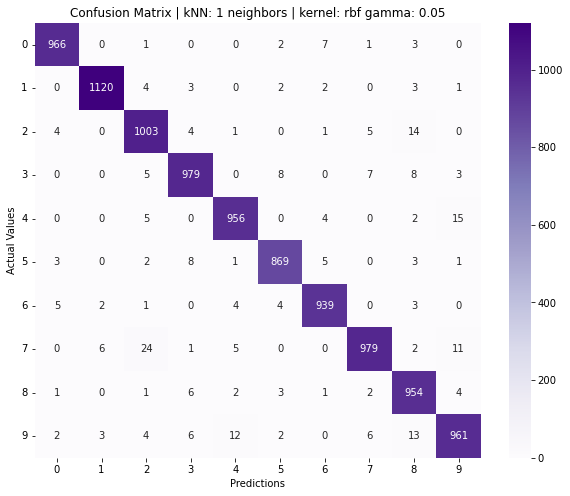
\includegraphics[width=0.6\linewidth]{mnist/confusion_matrix_knn.png}
    \caption{Confusion matrix για τη μέθοδο πλησιέστερων γειτόνων για τη βάση
    MNIST}
    \label{fig:mnist_confusion_knn}
\end{figure}

\begin{figure}[H]
    \centering

    \begin{subfigure}[t]{0.48\linewidth}
    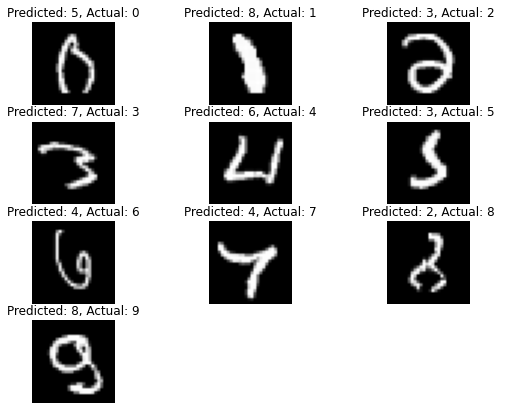
\includegraphics[width=\linewidth]{mnist/wrong_results_knn_1.png}
    \end{subfigure}
    \begin{subfigure}[t]{0.48\linewidth}
    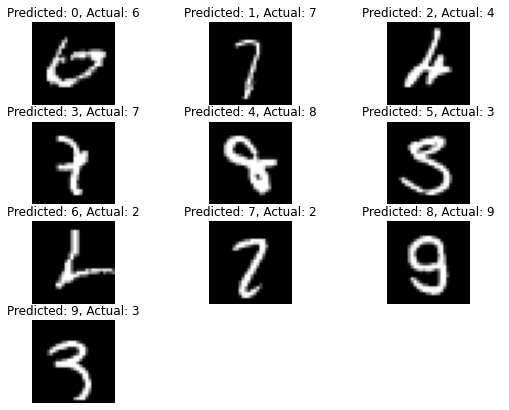
\includegraphics[width=\linewidth]{mnist/wrong_results_knn_2.png}
    \end{subfigure}

    \caption{Λάθος ταξινομήσεις του καλύτερου μοντέλου για τη μέθοδο
    πλησιέστερων γειτόνων και τη βάση MNIST}
    \label{fig:mnist_wrong_knn}
\end{figure}

\paragraph{Πλησιέστερου κέντρου κλάσης}

Στα \autoref{tab:mnist_train_final_nc} και \autoref{tab:mnist_test_final_nc}
παρουσιάζονται μετρικές και χρόνος εκτέλεσης του καλύτερου μοντέλου.

\begin{table}[H]
\centering
\begin{tabular}{|l|c|c|c|c|c|c|}
\hline
\textbf{Model}                                                    & \textbf{Accuracy} & \textbf{Precision} & \textbf{Recall} & \textbf{F1} & \textbf{KPCA+LDA Time (seconds)} & \textbf{Nearest Centroid Time} \\ \hline
\begin{tabular}[c]{@{}l@{}}kernel: rbf\\ gamma: 0.05\end{tabular} & 0,9145            & 0,9158             & 0,9145          & 0,9149      & 8818,2817                        & 0,0125                         \\ \hline
\end{tabular}
\caption{Αποτελέσματα καλύτερου μοντέλου πλησιέστερου κέντρου κλάσης στο σύνολο
    εκπαίδευσης για τη βάση MNIST}
\label{tab:mnist_train_final_nc}
\end{table}

\begin{table}[H]
\centering
\begin{tabular}{|l|c|c|c|c|c|c|}
\hline
\textbf{Model}                                                    & \textbf{Accuracy} & \textbf{Precision} & \textbf{Recall} & \textbf{F1} & \textbf{KPCA+LDA Time (seconds)} & \textbf{Nearest Centroid Time} \\ \hline
\begin{tabular}[c]{@{}l@{}}kernel: rbf\\ gamma: 0.05\end{tabular} & 0,9484            & 0,9487             & 0,9482          & 0,9482      & 8818,2817                        & 0,0125                         \\ \hline
\end{tabular}
\caption{Αποτελέσματα καλύτερου μοντέλου πλησιέστερου κέντρου κλάσης στο σύνολο
    ελέγχου για τη βάση MNIST}
\label{tab:mnist_test_final_nc}
\end{table}

Στο \autoref{fig:mnist_confusion_nc} φαίνεται το confusion matrix γι᾽ αυτό το
μοντέλο. Από το σχήμα αυτό παρατηρείται ότι οι περισσότερες εσφαλμένες
ταξινομήσεις γίνονται όταν:

\begin{itemize}
    \item Η πραγματική κλάση είναι {\bf7} ενώ το μοντέλο την ταξινομεί στη
        {\bf2}.
    \item Η πραγματική κλάση είναι {\bf7} ενώ το μοντέλο την ταξινομεί στη
        {\bf9}.
    \item Η πραγματική κλάση είναι {\bf9} ενώ το μοντέλο την ταξινομεί στη
        {\bf4}.
    \item Η πραγματική κλάση είναι {\bf2} ενώ το μοντέλο την ταξινομεί στη
        {\bf8}.
\end{itemize}

Από το \autoref{fig:mnist_wrong_nc} φαίνονται μερικές από τις λάθος ταξινομήσεις
του μοντέλου.

\begin{figure}[H]
    \centering
    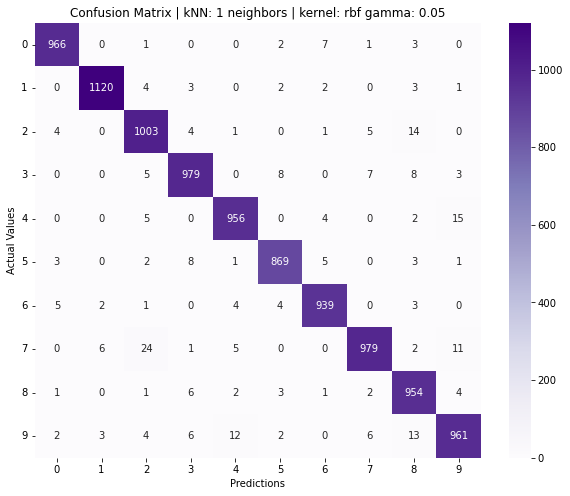
\includegraphics[width=0.6\linewidth]{mnist/confusion_matrix_knn.png}
    \caption{Confusion matrix για τη μέθοδο πλησιέστερου κέντρου κλάσης για τη
    βάση MNIST}
    \label{fig:mnist_confusion_nc}
\end{figure}

\begin{figure}[H]
    \centering

    \begin{subfigure}[t]{0.48\linewidth}
    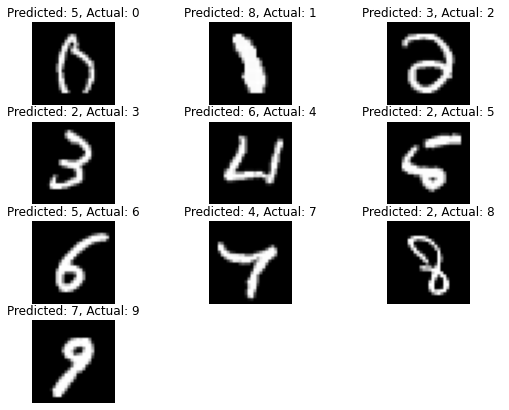
\includegraphics[width=\linewidth]{mnist/wrong_results_nc_1.png}
    \end{subfigure}
    \begin{subfigure}[t]{0.48\linewidth}
    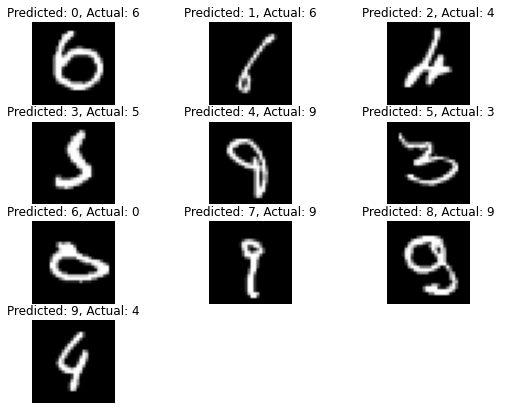
\includegraphics[width=\linewidth]{mnist/wrong_results_nc_2.png}
    \end{subfigure}

    \caption{Λάθος ταξινομήσεις του καλύτερου μοντέλου για τη μέθοδο
    πλησιέστερου κέντρου κλάσης και τη βάση MNIST}
    \label{fig:mnist_wrong_nc}
\end{figure}

\subsubsection{Cifar-10}

Το καλύτερο μοντέλο για τη βάση Cifar-10 είναι αυτό με RBF πυρήνα και $\gamma =
0.01$. Γι᾽ αυτό το μοντέλο εφαρμόζεται η μέθοδος KPCA plus LDA με τις βέλτιστες
παραμέτρους που αναφέρθηκαν και γίνεται ταξινόμηση με τη μέθοδο πλησιέστερων
γειτόνων και πλησιέστερου κέντρου κλάσης.

\paragraph{Πλησιέστερων γειτόνων}

Στα \autoref{tab:cifar_train_final_knn} και \autoref{tab:cifar_test_final_knn}
παρουσιάζονται μετρικές και χρόνος εκτέλεσης του καλύτερου μοντέλου.

\begin{table}[H]
\centering
\begin{tabular}{|l|c|c|c|c|c|c|c|}
\hline
\textbf{Model}                                                    & \textbf{Best n} & \textbf{Accuracy} & \textbf{Precision} & \textbf{Recall} & \textbf{F1} & \textbf{KPCA+LDA Time (seconds)} & \textbf{kNN Time} \\ \hline
\begin{tabular}[c]{@{}l@{}}kernel: rbf\\ gamma: 0.01\end{tabular} & 15              & 0,9992            & 0,9992             & 0,9992          & 0,9992      & 13608,5766                       & 5,3204            \\ \hline
\end{tabular}
\caption{Αποτελέσματα καλύτερου μοντέλου πλησιέστερων γειτόνων στο σύνολο
    εκπαίδευσης για τη βάση Cifar-10}
\label{tab:cifar_train_final_knn}
\end{table}

\begin{table}[H]
\centering
\begin{tabular}{|l|c|c|c|c|c|c|c|}
\hline
\textbf{Model}                                                    & \textbf{Best n} & \textbf{Accuracy} & \textbf{Precision} & \textbf{Recall} & \textbf{F1} & \textbf{KPCA+LDA Time (seconds)} & \textbf{kNN Time} \\ \hline
\begin{tabular}[c]{@{}l@{}}kernel: rbf\\ gamma: 0.01\end{tabular} & 15              & 0,449             & 0,5304             & 0,449           & 0,4499      & 13608,5766                       & 5,3204            \\ \hline
\end{tabular}
\caption{Αποτελέσματα καλύτερου μοντέλου πλησιέστερων γειτόνων στο σύνολο
    ελέγχου για τη βάση Cifar-10}
\label{tab:cifar_test_final_knn}
\end{table}

Στο \autoref{fig:cifar_confusion_knn} φαίνεται το confusion matrix γι᾽ αυτό το
μοντέλο. Από το σχήμα αυτό παρατηρείται ότι οι περισσότερες εσφαλμένες
ταξινομήσεις γίνονται όταν:

\begin{itemize}
    \item Η πραγματική κλάση είναι {\bf γάτα} ενώ το μοντέλο την ταξινομεί στη
        {\bf σκύλος}.
    \item Η πραγματική κλάση είναι {\bf πουλί} ενώ το μοντέλο την ταξινομεί στη
        {\bf ελάφι}.
    \item Η πραγματική κλάση είναι {\bf βάτραχος} ενώ το μοντέλο την ταξινομεί
        στη {\bf ελάφι}.
    \item Η πραγματική κλάση είναι {\bf φορτηγό} ενώ το μοντέλο την ταξινομεί στη
        {\bf αεροπλάνο}.
\end{itemize}

Στο \autoref{fig:cifar_wrong_knn} παρουσιάζονται μερικές λάθος ταξινομήσεις του
μοντέλου.

\begin{figure}[H]
    \centering
    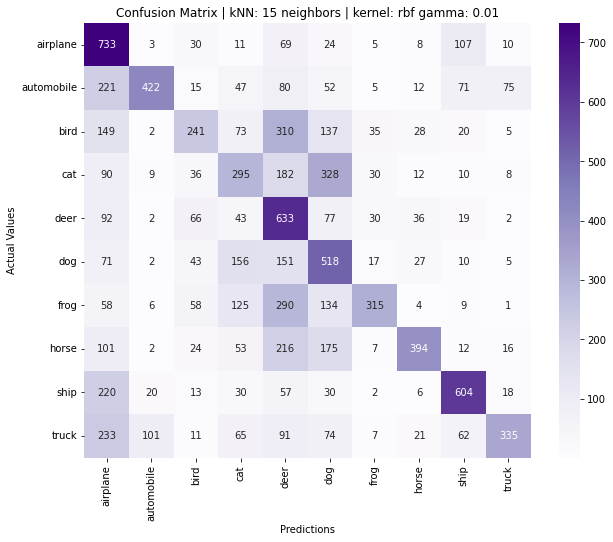
\includegraphics[width=0.6\linewidth]{cifar/confusion_matrix_knn.png}
    \caption{Confusion matrix για τη μέθοδο πλησιέστερων γειτόνων και τη βάση
    Cifar-10}
    \label{fig:cifar_confusion_knn}
\end{figure}

\begin{figure}[H]
    \centering

    \begin{subfigure}[t]{0.48\linewidth}
    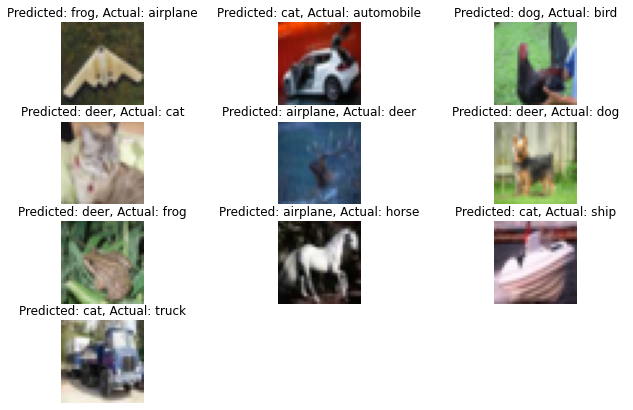
\includegraphics[width=\linewidth]{cifar/wrong_results_knn_1.png}
    \end{subfigure}
    \begin{subfigure}[t]{0.48\linewidth}
    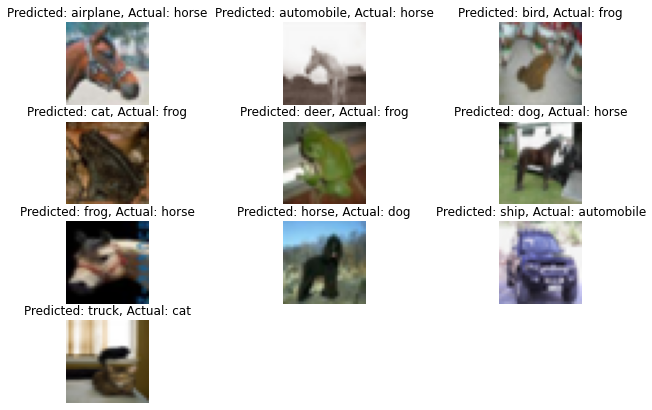
\includegraphics[width=\linewidth]{cifar/wrong_results_knn_2.png}
    \end{subfigure}

    \caption{Λάθος ταξινομήσεις του καλύτερου μοντέλου για τη μέθοδο
    πλησιέστερων γειτόνων και τη βάση Cifar-10}
    \label{fig:cifar_wrong_knn}
\end{figure}

\paragraph{Πλησιέστερου κέντρου κλάσης}

Στα \autoref{tab:cifar_train_final_nc} και \autoref{tab:cifar_test_final_nc}
παρουσιάζονται μετρικές και χρόνος εκτέλεσης του καλύτερου μοντέλου.

\begin{table}[H]
\centering
\begin{tabular}{|l|c|c|c|c|c|c|}
\hline
\textbf{Model}                                                    & \textbf{Accuracy} & \textbf{Precision} & \textbf{Recall} & \textbf{F1} & \textbf{KPCA+LDA Time (seconds)} & \textbf{Nearest Centroid Time} \\ \hline
\begin{tabular}[c]{@{}l@{}}kernel: rbf\\ gamma: 0.01\end{tabular} & 0,7629            & 0,7637             & 0,7629          & 0,7631      & 13608,5766                       & 0,0118                         \\ \hline
\end{tabular}
\caption{Αποτελέσματα καλύτερου μοντέλου πλησιέστερου κέντρου κλάσης στο σύνολο
    εκπαίδευσης για τη βάση Cifar-10}
\label{tab:cifar_train_final_nc}
\end{table}

\begin{table}[H]
\centering
\begin{tabular}{|l|c|c|c|c|c|c|}
\hline
\textbf{Model}                                                    & \textbf{Accuracy} & \textbf{Precision} & \textbf{Recall} & \textbf{F1} & \textbf{KPCA+LDA Time (seconds)} & \textbf{Nearest Centroid Time} \\ \hline
\begin{tabular}[c]{@{}l@{}}kernel: rbf\\ gamma: 0.01\end{tabular} & 0,4866            & 0,4899             & 0,4866          & 0,4808      & 13608,5766                       & 0,0118                         \\ \hline
\end{tabular}
\caption{Αποτελέσματα καλύτερου μοντέλου πλησιέστερου κέντρου κλάσης στο σύνολο
    ελέγχου για τη βάση Cifar-10}
\label{tab:cifar_test_final_nc}
\end{table}

Στο \autoref{fig:cifar_confusion_nc} φαίνεται το confusion matrix γι᾽ αυτό το
μοντέλο. Από το σχήμα αυτό παρατηρείται ότι οι περισσότερες εσφαλμένες
ταξινομήσεις γίνονται όταν:

\begin{itemize}
    \item Η πραγματική κλάση είναι {\bf γάτα} ενώ το μοντέλο την ταξινομεί στη
        {\bf σκύλος}.
    \item Η πραγματική κλάση είναι {\bf φορτηγό} ενώ το μοντέλο την ταξινομεί στη
        {\bf αυτοκινητιστικό} (automobile).
    \item Η πραγματική κλάση είναι {\bf γάτα} ενώ το μοντέλο την ταξινομεί στη
        {\bf βάτραχος}.
    \item Η πραγματική κλάση είναι {\bf ελάφι} ενώ το μοντέλο την ταξινομεί
        στη {\bf βάτραχος}.
\end{itemize}

Στο \autoref{fig:cifar_wrong_nc} παρουσιάζονται μερικές λάθος ταξινομήσεις του
μοντέλου.

\begin{figure}[H]
    \centering
    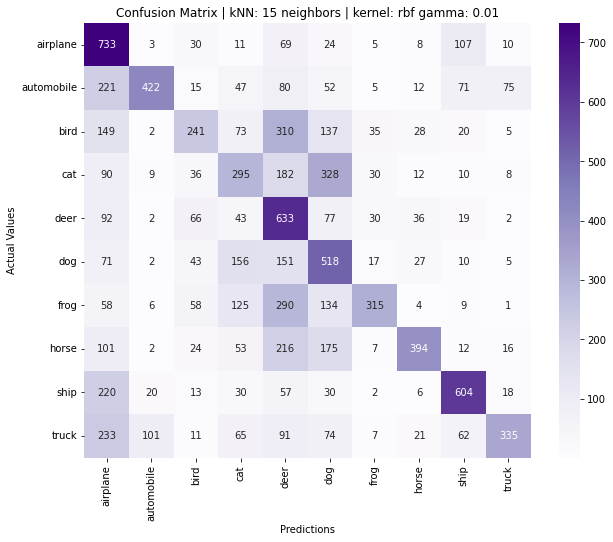
\includegraphics[width=0.6\linewidth]{cifar/confusion_matrix_knn.png}
    \caption{Confusion matrix για τη μέθοδο πλησιέστερου κέντρου κλάσης και τη
    βάση Cifar-10}
    \label{fig:cifar_confusion_nc}
\end{figure}

\begin{figure}[H]
    \centering

    \begin{subfigure}[t]{0.48\linewidth}
    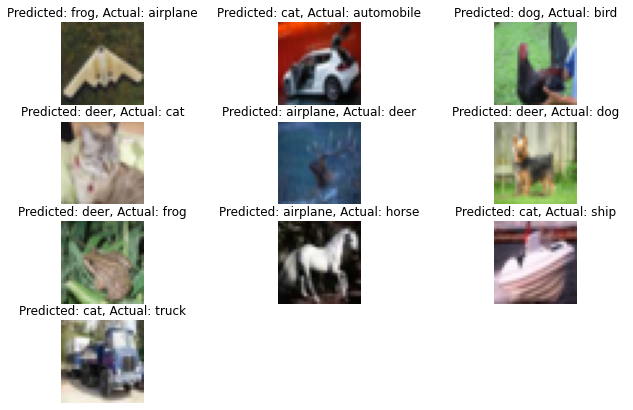
\includegraphics[width=\linewidth]{cifar/wrong_results_knn_1.png}
    \end{subfigure}
    \begin{subfigure}[t]{0.48\linewidth}
    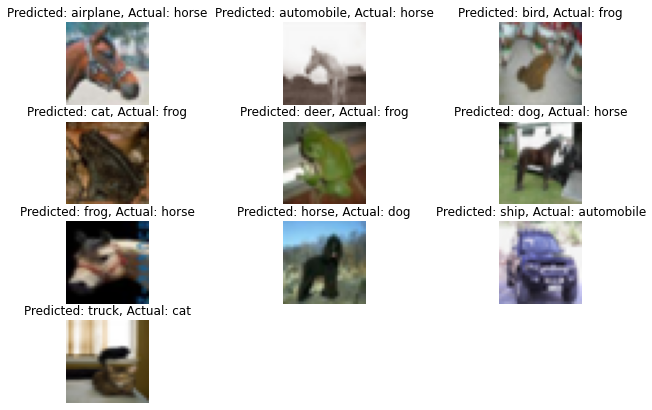
\includegraphics[width=\linewidth]{cifar/wrong_results_knn_2.png}
    \end{subfigure}

    \caption{Λάθος ταξινομήσεις του καλύτερου μοντέλου για τη μέθοδο
    πλησιέστερου κέντρου κλάσης και τη βάση Cifar-10}
    \label{fig:cifar_wrong_nc}
\end{figure}

\section{Σύγκριση με τα αποτελέσματα των SVMs}

Θα γίνει σύγκριση μεταξύ των προηγούμενων αποτελεσμάτων σε σχέση με τα
αποτελέσματα από τα SVMs. Θα πρέπει να γίνει η υπενθύμιση ότι το σύνολο
εκπαίδευσης της μεθόδου KPCA plus LDA είναι πολύ μικρότερο σε σχέση με το σύνολο
εκπαίδευσης που χρησιμοποιήθηκε στα SVMs. Παρόλα αυτά, θα παρουσιαστούν τα
καλύτερα αποτελέσματα και από τις δύο μεθόδους.

Όπως θα αναφερθεί και παρακάτω τα αποτελέσματα από την αρχιτεκτονική των SVMs
είναι καλύτερα και για τις δύο βάσεις. Ο χρόνος εκτέλεσης όμως είναι μικρότερος
για τα SVMs αν και στη μέθοδο KPCA plus LDA ο αριθμός των δηγμάτων που
χρησιμοποιήθηκαν για την εκπαίδευση είναι πολύ μικρότερος.

\subsection{MNIST}

Τα αποτελέσματα στο σύνολο ελέγχου για την αρχιτεκτονική του SVM είναι καλύτερα
και παρουσιάζονται στο \autoref{tab:mnist_svm_kpca}.

\begin{table}[H]
\centering
\begin{tabular}{|l|c|c|c|c|}
\hline
\textbf{Model} & \textbf{Accuracy} & \textbf{Precision} & \textbf{Recall} & \textbf{F1}\\ \hline
SVM & 0,9841 & 0,984 & 0,9841 & 0,984\\ \hline
KPCA+LDA & 0,9726 & 0,9726 & 0,9726 & 0,9725 \\ \hline
\end{tabular}
\caption{Αποτελέσματα για τα καλύτερα μοντέλα για τις αρχιτεκτονικές SVM και
    KPCA plus LDA στο σύνολο ελέγχου για τη βάση MNIST}
\label{tab:mnist_svm_kpca}
\end{table}

\subsection{Cifar-10}

Τα αποτελέσματα στο σύνολο ελέγχου για την αρχιτεκτονική του SVM είναι καλύτερα
και παρουσιάζονται στο \autoref{tab:cifar_svm_kpca}.

\begin{table}[H]
\centering
\begin{tabular}{|l|c|c|c|c|}
\hline
\textbf{Model} & \textbf{Accuracy} & \textbf{Precision} & \textbf{Recall} & \textbf{F1}\\ \hline
SVM & 0,56 & 0,5626 & 0,56 & 0,5607\\ \hline
KPCA+LDA & 0,4866 & 0,4899 & 0,4866 & 0,4808\\ \hline
\end{tabular}
\caption{Αποτελέσματα για τα καλύτερα μοντέλα για τις αρχιτεκτονικές SVM και
    KPCA plus LDA στο σύνολο ελέγχου για τη βάση Cifar-10}
\label{tab:cifar_svm_kpca}
\end{table}

\newpage
\begin{english}
\printbibliography[title=Βιβλιογραφία]
\end{english}


\end{document}
